% ============================================================
\chapter{Definizione dell'infrastruttura e delle Zone di Sicurezza}
% ============================================================

L'architettura di rete del sistema \textbf{BuySellChain} è stata progettata e segmentata seguendo i principi fondamentali dello standard internazionale IEC~62443. Questa suddivisione in zone logiche di sicurezza (\textit{Security Zones}) e condotti di comunicazione (\textit{Conduits}) permette di isolare i sistemi critici, limitare drasticamente i movimenti laterali di un eventuale attaccante in caso di compromissione perimetrale e applicare policy di accesso granulari basate sul principio del minimo privilegio (\textit{Least Privilege}).

% ------------------------------------------------------------
\section{Zona DMZ (Demilitarized Zone)}
% ------------------------------------------------------------

La DMZ funge da livello cuscinetto tra la rete pubblica (Internet) e la rete interna strettamente confinata. Il suo scopo è ricevere, filtrare e sanitizzare tutte le richieste provenienti dall'esterno prima che queste possano raggiungere i sistemi di validazione e persistenza dei dati.

\begin{table}[h]
\centering
\small
\renewcommand{\arraystretch}{1.4}
\begin{tabularx}{\textwidth}{>{\bfseries}p{3.5cm} X}
\toprule
\textbf{Componente} & \textbf{Descrizione e Funzione Architetturale} \\
\midrule
Reverse Proxy (NGINX) &
    Gestisce la terminazione TLS/SSL, isolando i server applicativi dall'esposizione diretta.
    Fornisce funzionalità di bilanciamento del carico e mitigazione base contro attacchi
    volumetrici (DDoS). \\[4pt]
Security Gateway (Backend) &
    Server applicativo sviluppato in Python/Flask. Agisce come \textit{Policy Enforcement Point}
    (PEP): valida i token JWT, implementa il controllo degli accessi (RBAC) e sanitizza gli
    input strutturali (JSON Schema) prima di invocare i comandi verso la blockchain. \\[4pt]
Gestore delle Sessioni &
    Modulo integrato nel Gateway per l'emissione, la validazione e la revoca dei JSON Web
    Token (JWT), gestendo le transizioni di stato dell'autenticazione in modalità stateless. \\
\bottomrule
\end{tabularx}
\caption{Componenti dell'infrastruttura situati nella Zona DMZ.}
\label{tab:dmz}
\end{table}

\newpage

% ------------------------------------------------------------
\section{Zona IT / Enterprise (Restricted Zone)}
% ------------------------------------------------------------

Questa zona, non accessibile direttamente dall'esterno, ospita i motori di persistenza, il sistema di consenso decentralizzato e i dati sensibili. Le comunicazioni in ingresso sono consentite esclusivamente dal Security Gateway tramite protocolli e porte rigorosamente definiti.

\begin{table}[h]
\centering
\small
\renewcommand{\arraystretch}{1.4}
\begin{tabularx}{\textwidth}{>{\bfseries}p{3.5cm} X}
\toprule
\textbf{Componente} & \textbf{Descrizione e Funzione Architetturale} \\
\midrule
Rete Hyperledger Fabric &
    Infrastruttura blockchain permissioned. Include gli \textit{Orderer Nodes} (per l'ordinamento
    crittografico dei blocchi) e i \textit{Peer Nodes} (per l'esecuzione dello Smart Contract e
    il mantenimento del Ledger distribuito). \\[4pt]
Smart Contract (Chaincode) &
    Codice eseguibile all'interno della rete Fabric che incapsula la logica di business
    immutabile (es.\ vincoli di rilancio, finestre temporali delle aste, transizioni di stato
    dell'asset). \\[4pt]
Client Lisp &
    Modulo software interno che agisce da intermediario tra il Security Gateway e la rete
    Fabric, occupandosi della firma delle transazioni tramite \textit{Membership Service
    Provider} (MSP). \\
\bottomrule
\end{tabularx}
\caption{Componenti dell'infrastruttura situati nella Zona IT / Enterprise.}
\label{tab:it-zone}
\end{table}

\newpage

% ============================================================
\section{Asset Inventory e Analisi delle Criticità}
% ============================================================

Il passo fondamentale per un'efficace modellazione delle minacce è l'identificazione e la classificazione degli asset. Di seguito vengono catalogati i componenti hardware, software e logici dell'infrastruttura BuySellChain. A ciascuno è assegnato un livello di criticità in base all'impatto di una potenziale violazione (in termini di disponibilità del servizio, integrità delle compravendite o riservatezza dei dati personali degli utenti).

\begin{table}[h]
\centering
\footnotesize
\renewcommand{\arraystretch}{1.4}
\begin{tabularx}{\textwidth}{>{\bfseries}p{2.8cm} p{2cm} p{1.6cm} X}
\toprule
\textbf{Asset} & \textbf{Tipo} & \textbf{Criticità} & \textbf{Dipendenze e Relazioni} \\
\midrule
Smart Contract (Chaincode) & Software & Critica &
    Dipende direttamente dal meccanismo di consenso di Fabric. Una compromissione logica
    altera irreversibilmente l'esito delle aste. \\[4pt]
Ledger Distribuito & Dati & Critica &
    Dipende dall'integrità dei Peer Nodes e dalle identità MSP. Contiene la \textit{provenance}
    e la proprietà legale degli asset immobiliari. \\[4pt]
Security Gateway (API) & Applicativo & Alta &
    Punto di esposizione pubblico verso la blockchain: valida l'autenticazione, applica RBAC
    e sanitizza gli input prima di invocare il Client Lisp. \\[4pt]
Chiavi Segrete & Crittografia & Estrema &
    Risiedono in memoria nel Security Gateway. Se esfiltrate, permettono a un attaccante di
    forgiare tag e sessioni valide, compromettendo la sicurezza generale del sistema. \\[4pt]
Frontend (Client Web) & Interfaccia & Media &
    Dipende dalla disponibilità del Security Gateway. Vulnerabile ad attacchi lato client
    (XSS, CSRF) ma non contiene logica di business fidata. \\[4pt]
API Catasto (Sistema Terzo) & Servizio Esterno & Alta &
    Dipende dall'ISP e dalle CA pubbliche. Utilizzato per certificare l'esistenza degli
    immobili; la sua indisponibilità blocca la creazione di nuove aste. \\
\bottomrule
\end{tabularx}
\caption{Inventario dettagliato degli asset del sistema BuySellChain con mappatura delle dipendenze.}
\label{tab:asset-inventory}
\end{table}

% ------------------------------------------------------------
\subsection{Endpoint del Security Gateway}
% ------------------------------------------------------------

La tabella seguente dettaglia gli endpoint esposti dal Security Gateway, classificandoli
come asset applicativi distinti in base alla loro superficie di attacco e criticità.

\begin{table}[h]
\centering
\footnotesize
\renewcommand{\arraystretch}{1.4}
\begin{tabularx}{\textwidth}{>{\bfseries}p{3.2cm} p{2cm} p{1.6cm} X}
\toprule
\textbf{Endpoint} & \textbf{Tipo} & \textbf{Criticità} & \textbf{Note} \\
\midrule
\texttt{GET/POST /admin} & Applicativo & Critica &
    Accesso riservato ad amministratori. Esposto a privilege escalation e a tentativi di
    accesso non autorizzato; richiede autenticazione forte e audit logging. \\[4pt]
\texttt{GET/POST /assets} & Applicativo & Media &
    Gestione degli asset immobiliari. Vulnerabile a injection nei campi descrittivi e
    a enumerazione non autorizzata degli asset altrui. \\[4pt]
\texttt{GET/POST /auctions} & Applicativo & Media &
    Creazione e consultazione delle aste. La creazione dipende dall'API Catasto; la sua
    indisponibilità blocca interamente il flusso di onboarding degli immobili. \\[4pt]
\texttt{GET/POST /bids} & Applicativo & Media &
    Invio e lettura delle offerte. Un picco anomalo di richieste POST può saturare
    il server o sovraccaricare la blockchain (DoS applicativo). \\[4pt]
\texttt{POST /auth} & Applicativo & Alta &
    Emissione e validazione dei JWT. Bersaglio primario di credential stuffing, brute
    force e session forgery; richiede rate limiting e blocco per IP anomali. \\
\bottomrule
\end{tabularx}
\caption{Endpoint del Security Gateway: classificazione per tipo e criticità.}
\label{tab:endpoints}
\end{table}

\newpage

% ============================================================
\section{Superficie Osservabile, Inferenza e Vettori di Attacco}
% ============================================================

La superficie osservabile rappresenta tutto ciò che un potenziale attaccante o un analista può dedurre dall'esterno dell'infrastruttura semplicemente intercettando il traffico di rete, analizzando i metadati delle comunicazioni o interagendo con le interfacce pubbliche.

Mappare questi elementi è cruciale per comprendere quali informazioni il sistema espone (anche involontariamente) e come anomalie o deviazioni comportamentali possano fungere da indicatori per formulare ipotesi di attacco. La tabella seguente unifica le osservazioni della superficie con le relative inferenze e i vettori di minaccia derivati (in linea con la metodologia STRIDE).

\begin{table}[h]
\centering
\footnotesize
\renewcommand{\arraystretch}{1.5}
\begin{tabularx}{\textwidth}{>{\bfseries}p{2.5cm} X X X}
\toprule
\textbf{Asset Target} & \textbf{Cosa si osserva (Sintomo)} & \textbf{Cosa si inferisce (Ipotesi)} & \textbf{Possibile Attacco (Minaccia)} \\
\midrule
Endpoint \texttt{/auth/login} &
    Picco anomalo di richieste POST (es.\ centinaia al secondo) provenienti da IP eterogenei
    o singole subnet. &
    L'attaccante sta testando liste di credenziali pre-esfiltrate o tentando di forzare
    una password. &
    \textbf{Credential Stuffing} o \textbf{Brute Force} (Spoofing). \\[4pt]
Endpoint \texttt{/admin/users} &
    Picco anomalo di richieste GET provenienti da IP eterogenei o singole subnet. &
    Tentativo di enumerare gli utenti del sistema. &
    \textbf{Enumeration}. \\[4pt]
Endpoint \texttt{/bids}, \texttt{/auctions}, \texttt{/assets} &
    Picco di richieste POST agli endpoint di creazione dati. &
    Tentativo di saturare il server oppure sovraccaricare la blockchain. &
    \textbf{Denial of Service} (DoS) applicativo o \textbf{Overflood}. \\[4pt]
Security Gateway (API) &
    Caratteri di escape insoliti, cicli annidati o tentativi di iniezione nei payload JSON
    in ingresso. &
    L'attaccante cerca di bypassare il parser per eseguire comandi diretti sul Client Lisp. &
    \textbf{Lisp Command Injection}. \\[4pt]
Sessioni Utente (JWT) &
    Modifica del payload Base64 del JWT (es.\ alterazione del campo \texttt{role} da
    \textit{Bidder} ad \textit{Admin}). &
    Un utente malintenzionato sta testando la robustezza dell'algoritmo di firma HMAC. &
    \textbf{Privilege Escalation} o \textbf{Session Forgery}. \\[4pt]
API Catasto (connessioni in uscita) &
    Traffico anomalo dal Security Gateway verso IP sconosciuti al di fuori dei domini
    governativi previsti. &
    Il Gateway è stato compromesso e sta esfiltrando dati, oppure è vittima di un attacco SSRF. &
    \textbf{Server-Side Request Forgery} o \textbf{Data Exfiltration} (Information Disclosure). \\[4pt]
Frontend (Interfaccia) &
    Inserimento di tag HTML o script JavaScript nei campi descrittivi degli immobili
    in vendita. &
    Ricerca di vulnerabilità nella sanitizzazione lato server dei template Jinja2. &
    \textbf{Cross-Site Scripting (XSS)} e furto di token. \\
\bottomrule
\end{tabularx}
\caption{Threat Model unificato: dalla superficie osservabile all'inferenza dell'attacco.}
\label{tab:threat-model}
\end{table}

\newpage

% ============================================================
\section{Grafo dell'Infrastruttura e Flussi di Comunicazione}
% ============================================================

Per agevolare l'analisi dei rischi e l'implementazione dei controlli di sicurezza, viene presentata la topologia dei flussi di rete. Questa scomposizione evidenzia i nodi di origine e destinazione, i confini di trust attraversati, i protocolli crittografici necessari e l'intensità fisiologica attesa per ciascun condotto (utile a stabilire una \textit{baseline} comportamentale per i sistemi di Intrusion Detection).

Ogni deviazione da questi flussi autorizzati (ad esempio, il Reverse Proxy NGINX che tenta di comunicare direttamente con la blockchain) deve essere considerata un'anomalia severa.

\begin{figure}[H]
    \centering
    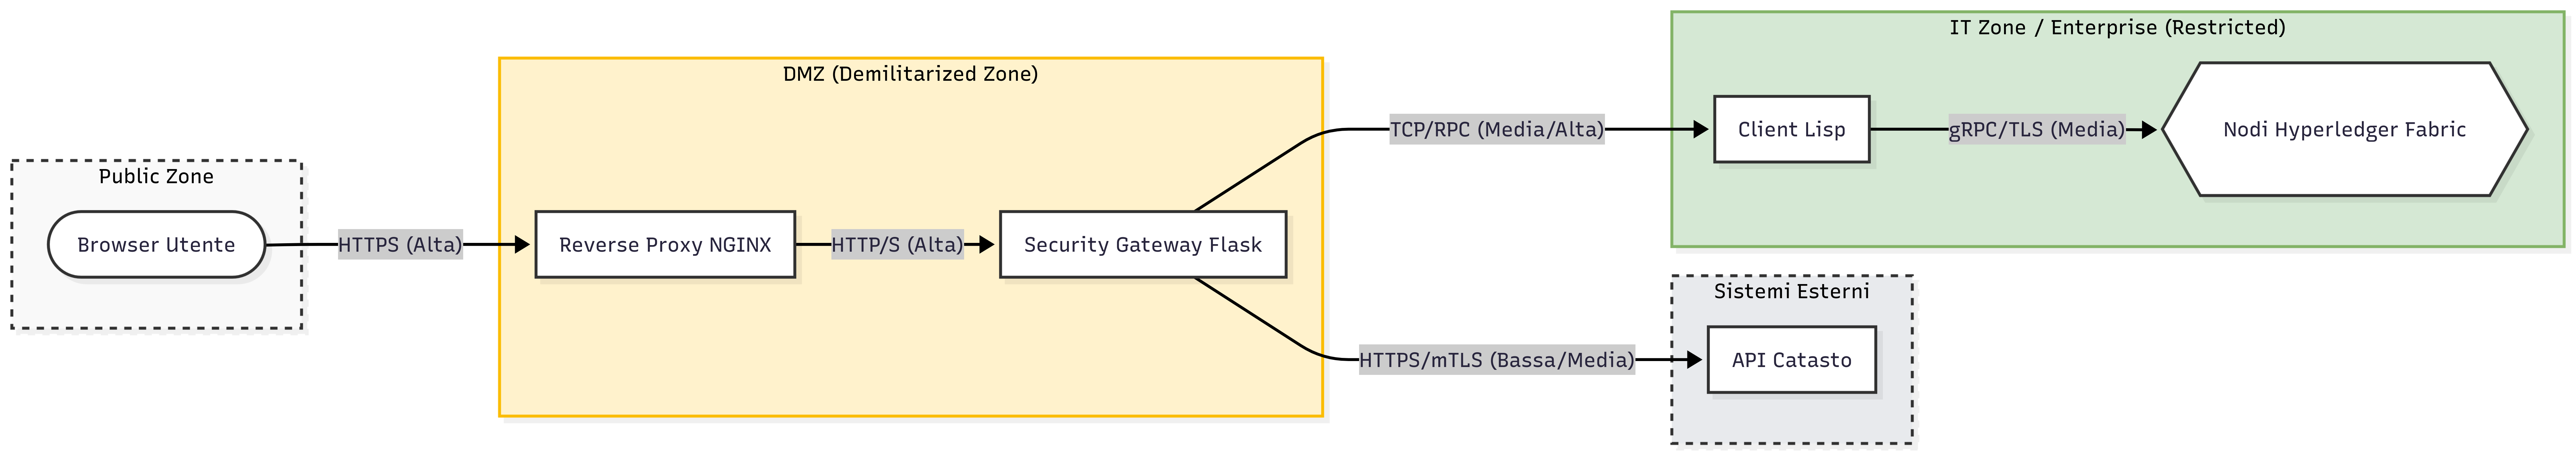
\includegraphics[width=1\textwidth]{images/threatmodelbuysellchaingraph.png}
    \caption{Grafo dell'infrastruttura BuySellChain con zone di sicurezza e flussi autorizzati.}
    \label{fig:graph}
\end{figure}

\begin{table}[h]
\centering
\footnotesize
\renewcommand{\arraystretch}{1.4}
\begin{tabularx}{\textwidth}{p{2.4cm} p{2.4cm} p{1.6cm} p{1.6cm} X}
\toprule
\textbf{Sorgente} & \textbf{Destinazione} & \textbf{Protocollo} & \textbf{Frequenza} & \textbf{Motivazione / Logica di Business} \\
\midrule
Browser Utente &
    Reverse Proxy (DMZ) & HTTPS & Alta &
    Navigazione piattaforma, consultazione grid aste, login e invio offerte. Traffico cifrato TLS~1.3. \\[4pt]
Reverse Proxy &
    Security Gateway & HTTP/S & Alta &
    Inoltro delle richieste decifrate (o ri-cifrate internamente) verso il server Flask per l'elaborazione. \\[4pt]
Security Gateway &
    Client Lisp (IT Zone) & TCP & Media/Alta &
    Traduzione delle chiamate REST in primitive (\texttt{AddKV}, \texttt{GetKV}) per l'interazione con la blockchain. \\[4pt]
Client Lisp &
    Nodi Fabric (IT Zone) & gRPC/TLS & Media &
    Invocazione dello Smart Contract, proposta di transazioni e interrogazione dello stato del Ledger. \\[4pt]
Security Gateway &
    API Catasto (Esterno) & HTTPS/mTLS & Bassa/Media &
    Chiamata sincrona per la certificazione e la validazione dei dati di un immobile in fase di creazione asta. \\
\bottomrule
\end{tabularx}
\caption{Mappatura dettagliata dei flussi di comunicazione autorizzati (Conduits) tra gli asset.}
\label{tab:conduits}
\end{table}

\newpage

% ============================================================
\section{Dall'Architettura alla Baseline Comportamentale (Operating Envelope)}
% ============================================================

L'obiettivo di questa fase è usare la topologia di BuySellChain per definire cosa costituisce un comportamento di rete \textit{normale}.
La normalità non è un punto singolo, ma un inviluppo operativo continuo (\textit{operating envelope}).
La classificazione degli eventi deve quindi distinguere tra \textbf{Normal}, \textbf{Deviazione Lieve}, \textbf{Deviazione Forte} e \textbf{Unknown}.

% ------------------------------------------------------------
\subsection{Definizione della Baseline Qualitativa}
% ------------------------------------------------------------

Le comunicazioni attese vengono modellate come relazioni lecite tra asset, con frequenza temporale e intensità prevista.

\begin{table}[h]
\centering
\small
\renewcommand{\arraystretch}{1.4}
\begin{tabularx}{\textwidth}{>{\bfseries}p{3.8cm} p{2cm} p{1.6cm} X}
\toprule
\textbf{Relazione Normale} & \textbf{Quando} & \textbf{Intensità} & \textbf{Note} \\
\midrule
Frontend Web $\rightarrow$ Security Gateway &
    Sempre & Alta &
    Navigazione utenti, login, invio offerte. \\[4pt]
Security Gateway $\rightarrow$ Rete Fabric (via Client Lisp) &
    Sempre & Media &
    Invocazione Smart Contract per registrazione aste e offerte. \\[4pt]
Security Gateway $\rightarrow$ API Catasto &
    Giorno/Notte & Bassa/Media &
    Verifica validità immobili, chiamate asincrone e sincrone. \\[4pt]
Client esterno $\rightarrow$ Server Gateway &
    Mai & Nulla &
    Deviazione topologica grave. Client non-browser che tentano di invocare
    direttamente lo Smart Contract. \\[4pt]
\midrule
\multicolumn{4}{l}{\textit{Flussi utente (Seller/Buyer) — baseline applicativa}} \\
\midrule
Login/Registrazione $\rightarrow$ Crea Asset $\rightarrow$ Crea Asta &
    Sì & Normale &
    Flusso canonico del venditore: autenticazione, onboarding immobile, apertura asta. \\[4pt]
Login/Registrazione $\rightarrow$ Crea Asta &
    Sì & Normale &
    Flusso abbreviato se l'asset è già presente nel ledger. \\[4pt]
Home Page (no login) $\rightarrow$ Crea Asta / Crea Asset &
    No & Deviazione &
    Accesso a risorse protette senza autenticazione.
    \textbf{Contromisura:} redirect al login o risposta \texttt{403 Forbidden}. \\
\bottomrule
\end{tabularx}
\caption{Baseline qualitativa dei flussi leciti e applicativi (Operating Envelope).}
\label{tab:baseline}
\end{table}

\newpage

\chapter{Logger}

Per completare il modello di minaccia, è necessario definire un sistema di logging centralizzato che raccolga i dati di telemetria da tutti i componenti critici (Security Gateway, Client Lisp, Nodi Fabric) e li normalizzi in un formato standardizzato (es.\ JSON con timestamp ISO8601, ID transazione, livello di severità).
Questi log devono essere arricchiti con metadati contestuali (es.\ geolocalizzazione IP, user agent, payload size) per facilitare l'analisi comportamentale e la correlazione degli eventi. Il sistema di logging deve essere progettato per resistere a tentativi di manomissione (es.\ log immutabili, firma digitale dei log) e per supportare query ad-hoc per l'investigazione post-incident.

Come vedremo, il sistema di logging scrive i record in blockchain, garantendo così l'immutabilità e la tracciabilità completa degli eventi di sicurezza. Questo approccio innovativo consente di superare le limitazioni dei tradizionali sistemi di logging centralizzati, offrendo una soluzione altamente resistente alla manomissione e alla perdita dei dati, e facilitando l'analisi forense in caso di incidenti di sicurezza.

Prima di definire il sistema di logging, abbiamo effettuato una migrazione della tabella \texttt{Users}, dal database off-chain Postgres, alla blockchain Hyperledger Fabric. Questa migrazione è stata necessaria per garantire la coerenza e l'integrità dei dati degli utenti, sfruttando le caratteristiche di immutabilità e decentralizzazione della blockchain. La tabella \texttt{Users} ora risiede all'interno della blockchain, consentendo una gestione più sicura e trasparente delle informazioni degli utenti, e facilitando l'implementazione di meccanismi di autenticazione e autorizzazione basati su identità digitali registrate sulla blockchain. 

\section{Definizione Sistema di Logging}

Inannzitutto è stato necessario definire quali metadati devono essere raccolti nei log per garantire un'analisi efficace degli eventi di sicurezza. I log devono includere informazioni quali timestamp, livello di criticità, geolocalizzazione IP, user agent, metodo HTTP e payload size. Questi metadati consentono di contestualizzare gli eventi e facilitano l'identificazione di pattern sospetti o anomalie nel comportamento degli utenti o dei sistemi.

Memorizzare in \textbf{chiaro} l'IP e lo user agent di chi interagisce con il sistema è controproducente per la privacy degli utenti, ma è necessario per l'analisi comportamentale e la correlazione degli eventi. Per mitigare questo rischio, i log vengono cifrati prima di essere scritti sulla blockchain, utilizzando una chiave simmetrica gestita in modo sicuro all'interno del Security Gateway. In questo modo, anche se i log sono immutabili e trasparenti sulla blockchain, le informazioni sensibili rimangono protette e accessibili solo agli operatori autorizzati che dispongono della chiave di decrittazione.

Di seguito, è mostrata la struttura dei log:

\begin{lstlisting}[language=json, basicstyle=\scriptsize\ttfamily, breaklines=true]
{

    "id": hash(description, created_at, level, from_ip, user_agent, method, payload_size),
    "description": MessaggeType,
    "created_at": timestamp,
    "level": INFO/ALERT,
    "from_ip": AES-256-GCM(source IPv4),
    "method": HTTP method,
    "user_agent": AES-256-GCM(useragent),
    "payload_size": N Kb size of payload
}
\end{lstlisting}

In particolare, il logger tiene traccia delle seguenti azioni:
\begin{itemize}
    \item \textbf{Login/Registrazione}: ogni tentativo di autenticazione, riuscito o fallito, viene registrato con il relativo user agent e IP di origine. Inoltre, viene segnalato ogni nuovo utente registrato nel sistema.
    \item \textbf{Creazione Asta}: quando un utente crea una nuova asta, viene loggato l'ID dell'asta, l'ID dell'utente e i dettagli dell'immobile.
    \item \textbf{Creazione Asset}: quando un utente crea una nuovo asset, viene loggato l'ID dell'asset, l'ID dell'utente e i dettagli dell'immobile.
    \item \textbf{Offerte}: ogni offerta fatta su un'asta viene registrata con l'ID dell'offerta, l'ID dell'utente, l'importo e l'ID dell'asta.
    \item \textbf{Errori e Anomalie}: qualsiasi errore del sistema o comportamento anomalo (es.\ tentativi di accesso non autorizzati) viene loggato con un livello di criticità adeguato (INFO, ALERT).
\end{itemize}

Come accennato sopra, i campi \texttt{from\_ip} e \texttt{user\_agent} vengono cifrati prima di essere memorizzati sulla blockchain, garantendo così la protezione della privacy degli utenti pur mantenendo la capacità di analizzare i log per identificare comportamenti sospetti o pattern di attacco. Solo l'admin, il quale ha accesso alle api di lettura dei log è in grado di leggere in chiaro questi campi, e solo in caso di necessità di investigazione post-incident.

\newpage

\section{Esempi di Log e Analisi Comportamentale}

Di seguito, vediamo alcuni esempi:

\begin{description}

    \item[Log Cifrato in Blockchain]
    Se eseguita una \texttt{GetKV} per leggere un log relativo alla registrazione di un
    nuovo utente, il record restituito sarà simile al seguente (con i campi sensibili cifrati):

\begin{lstlisting}[language=json, basicstyle=\scriptsize\ttfamily, breaklines=true]
{
    "success": true,
    "message": "Ok",
    "answer": {
        "value": {
            "id": "6a8e249114664e905f84d83d7c992a860e950f5baf04894679581a05bd69d9e1",
            "description": "Nuovo utente registrato: user123",
            "created_at": "2026-05-15T11:47:53.512788",
            "level": "INFO",
            "from_ip": "lIBpH+5m+OHAsrUVwVV1l9i0Yvu2KSqVGk8zxymgJpVQqOFKP70dRgg=",
            "user_agent": "2j0pqAPMUAad5KVGvUzR8gc9ZhmmWz3uYKvFNLeMaCe0mSQeuoY9ykcAcUAIenUC",
            "method": "POST"
            "payload_size": 45
        },
        "key": [
            "6a8e249114664e905f84d83d7c992a860e950f5baf04894679581a05bd69d9e1"
        ],
        "class": "Logs"
    }
}
\end{lstlisting}

    \item[Log Decifrato per Analisi]
    Se l'admin esegue una query per leggere i log, i campi cifrati vengono decifrati e
    restituiti in chiaro, consentendo di analizzare le informazioni per identificare
    eventuali anomalie o pattern sospetti:

\begin{lstlisting}[language=json, basicstyle=\scriptsize\ttfamily, breaklines=true]
{
    "created_at": "2026-05-15T11:47:53.512788",
    "from_ip": "127.0.0.1",
    "id": "6a8e249114664e905f84d83d7c992a860e950f5baf04894679581a05bd69d9e1",
    "level": "INFO",
    "message": "Nuovo utente registrato: user123",
    "method": "POST",
    "payload_size": 45,
    "user_agent": "Mozilla/5.0 (X11; Linux x86_64; rv:150.0) Gecko/20100101 Firefox/150.0"
}
\end{lstlisting}

\end{description}

\newpage

\subsection{User Agent Metadata Role}

Un metadato fondamentale per l'analisi comportamentale è lo \texttt{user\_agent}. Questo ci dice da quale software/client vengono fatte le richieste al server. Se vediamo un user agent insolito (es.\ un tool di pen testing o un bot), questo può essere un indicatore di attività malevola. Ad esempio, se notiamo un picco di richieste con user agent "sqlmap" o "Nmap", potremmo inferire che qualcuno sta cercando di identificare vulnerabilità nel sistema. Allo stesso modo, se vediamo user agent che non corrispondono a browser comuni (es.\ "curl/7.68.0"), questo potrebbe indicare tentativi di accesso automatizzati o scriptati, che potrebbero essere utilizzati per attacchi di forza bruta o scraping dei dati.

\begin{lstlisting}[language=json, basicstyle=\scriptsize\ttfamily, breaklines=true]
{
    "created_at": "2026-05-15T12:41:24.896036",
    "from_ip": "127.0.0.1",
    "id": "9f1b99fc04ee6a489da4901ab9eb226cfdbf930877f7422752c21a609a7d581a",
    "level": "ALERT",
    "message": "Accesso non autorizzato /auctions/create",
    "method": "GET",
    "payload_size": 0,
    "user_agent": "curl/8.15.0"
}
\end{lstlisting}

Come possiamo vedere nell'esempio sopra, il log indica un tentativo di accesso non autorizzato all'endpoint \texttt{/auctions/create} utilizzando l'user agent "curl/8.15.0". Questo potrebbe essere un indicatore di un attacco automatizzato e dovrebbe essere investigato ulteriormente per determinare se si tratta di un'attività malevola o di un errore legittimo.

Inoltre, questo log ci dice anche che all' endpoint \texttt{/auctions/create} è stato fatto l'accesso senza autenticazione, il che è una deviazione dalla baseline operativa definita in precedenza, dove l'accesso a questo endpoint dovrebbe essere consentito solo agli utenti autenticati. Questo tipo di deviazione è un chiaro indicatore di un potenziale attacco e dovrebbe essere trattato con la massima attenzione.

\section{Monitoraggio Autenticazione \& Admin}

Il sistema di logging tiene traccia di tutti i tentativi di autenticazione, sia riusciti che falliti. Questo è fondamentale per identificare potenziali attacchi di forza bruta o credential stuffing. Ad esempio, se vediamo un picco di tentativi di login falliti da un singolo IP o da una serie di IP correlati, questo potrebbe indicare un attacco in corso.

Inoltre, il sistema di logging consente di monitorare le tendenze nel tempo, identificando periodi di attività sospetta o anomalie nei pattern di autenticazione. Ad esempio, se vediamo un aumento improvviso dei tentativi di login durante un periodo in cui normalmente ci sarebbe poca attività, questo potrebbe essere un indicatore di un attacco in corso.

Per non dare troppe informazioni nel caso in cui la blockchain venga compromessa, i log di autenticazione falliti conterranno solo un messaggio generico che indica un tentativo di login fallito. In questo modo, anche se un attaccante riesce ad accedere ai log, non avrà informazioni dettagliate sui tentativi di autenticazione falliti, riducendo il rischio di ulteriori attacchi basati su queste informazioni.

Infine, il sistema di logging consente di monitorare le attività degli amministratori, registrando ogni azione eseguita dagli utenti con privilegi elevati. Questo è fondamentale per identificare potenziali abusi di privilegi o attività sospette da parte degli amministratori stessi. Ad esempio, se vediamo un amministratore che accede a dati sensibili o esegue azioni non autorizzate, questo potrebbe essere un indicatore di un abuso di privilegi o di un attacco interno.

% % ------------------------------------------------------------
% \subsection{Finestra di Telemetria Osservata (Dataset di Esempio)}
% % ------------------------------------------------------------

% Si considera una finestra temporale campione con log estratti da firewall e Security Gateway.

% \begin{table}[h]
% \centering
% \footnotesize
% \renewcommand{\arraystretch}{1.35}
% \begin{tabularx}{\textwidth}{p{1.2cm} p{3.2cm} p{2.8cm} p{1.4cm} p{1cm} X}
% \toprule
% \textbf{Time} & \textbf{Source} & \textbf{Dest} & \textbf{Proto} & \textbf{Pkts} & \textbf{Status} \\
% \midrule
% 10:15 & Frontend Web (IP vari)          & Security Gateway         & HTTPS & 340  & ok \\
% 10:16 & Security Gateway                & DB Off-Chain             & TCP   & 510  & ok \\
% 10:17 & Security Gateway                & API Catasto              & HTTPS & 15   & ok \\
% 10:18 & IP Pubblico (sconosciuto)       & DB Off-Chain             & TCP   & 45   & fail \\
% 10:20 & Frontend Web (singolo IP)       & Security Gateway         & HTTPS & 850  & retry \\
% 03:05 & Security Gateway                & Backup Storage           & TCP   & 1500 & ok \\
% 03:10 & Security Gateway                & IP Pubblico (sconosciuto)& HTTPS & 2200 & ok \\
% \bottomrule
% \end{tabularx}
% \caption{Finestra di telemetria osservata per la classificazione delle deviazioni.}
% \label{tab:telemetria}
% \end{table}

% % ------------------------------------------------------------
% \subsection{Valutazione Deviazioni e Classificazione}
% % ------------------------------------------------------------

% Gli eventi non pienamente compatibili con la baseline vengono classificati con severità e motivazione.

% \begin{table}[h]
% \centering
% \footnotesize
% \renewcommand{\arraystretch}{1.4}
% \begin{tabularx}{\textwidth}{>{\bfseries}p{3cm} p{1.5cm} p{1.2cm} p{1.8cm} X}
% \toprule
% \textbf{Evento} & \textbf{Compatibile} & \textbf{Score} & \textbf{Classificazione} & \textbf{Dato utile (giustificazione)} \\
% \midrule
% 10:18 IP Pubblico $\rightarrow$ DB &
%     No & Forte & Attacco &
%     Log firewall: violazione grave della segmentazione. Il DB non deve ricevere traffico
%     diretto dall'esterno. \\[4pt]
% 10:20 Frontend $\rightarrow$ Gateway &
%     No & Medio & Fault / Attacco &
%     Log autenticazione API: anomalia volumetrica da singolo IP. Possibile credential
%     stuffing oppure errore client. \\[4pt]
% 03:05 Gateway $\rightarrow$ Backup &
%     Parziale & Lieve & Unknown &
%     Log schedulazione: trasferimento massivo atteso di notte, ma senza audit completo
%     resta non conclusivo. \\[4pt]
% 03:10 Gateway $\rightarrow$ IP Sconosciuto &
%     No & Forte & Attacco &
%     Ispezione connessioni: invio dati verso destinazione esterna non censita. Forte
%     indicatore di data exfiltration. \\
% \bottomrule
% \end{tabularx}
% \caption{Classificazione delle deviazioni rispetto alla baseline comportamentale.}
% \label{tab:deviazioni}
% \end{table}

% \newpage

% % ------------------------------------------------------------
% \subsection{Debrief Finale di Sicurezza}
% % ------------------------------------------------------------

% \paragraph{Asset più critico e deviazione più grave.}
% L'asset più critico resta lo \textbf{Smart Contract} su Fabric, poiché governa transazioni irreversibili di valore e proprietà.
% Le deviazioni più gravi osservate sono:
% \begin{itemize}
%     \item \texttt{03:10 Gateway $\rightarrow$ IP Sconosciuto}
%     \item \texttt{10:18 IP Pubblico $\rightarrow$ DB}
% \end{itemize}
% Entrambe indicano un potenziale data breach e il fallimento dei controlli perimetrali di base.

% \paragraph{Deviazione più ambigua.}
% \texttt{10:20 Frontend $\rightarrow$ Gateway} è ambigua: può essere un \textit{fault} applicativo (retry anomali) oppure un brute-force mirato. Senza log applicativi dettagliati, la decisione non è deterministica.

% \paragraph{Quando la risposta corretta è ``Unknown''.}
% Nel caso \texttt{03:05 Gateway $\rightarrow$ Backup}, il volume elevato notturno è coerente con job leciti di backup, ma in assenza di evidenze di audit la classificazione prudente resta \textbf{Unknown} per ridurre i falsi positivi.

% \paragraph{Controllo by-design prioritario.}
% La \textbf{Network Segmentation} rigorosa (DMZ + reti virtuali isolate) riduce i falsi negativi e limita il \textit{blast radius}. In questo modello, eventi come \texttt{IP Pubblico $\rightarrow$ DB} devono essere bloccati nativamente dal perimetro (\textit{default deny}).

% \begin{quote}
% \itshape
% ``Detection non significa indovinare attacchi. Significa ridurre l'incertezza fino a una decisione difendibile.''
% \end{quote}

